\documentclass[10pt]{article}
\usepackage[utf8]{inputenc}
\usepackage{parskip}
\usepackage[a4paper, margin=1.5in]{geometry}
\usepackage{graphicx}
\usepackage{hyperref}

\title{Task 0 Report}
\date{17/10/2019}
\author{Federico Fregosi, Mirko Laruina,\\
        Riccardo Mancini, Gianmarco Petrelli}

\begin{document}
\pagenumbering{gobble}
\maketitle
\vfill
% \setcounter{tocdepth}{1}
\tableofcontents
\vfill
\clearpage
\setcounter{page}{1}
\pagenumbering{arabic}

\section{Specifications}
\subsection{Application overview}
The application is a messaging system where registered users can create an 
account, exchange text messages and make groups.

A registered user can initiate a chat with another user, create a new group chat
(of which he becomes the admin) and send messages to the chats he belongs to,
as well as receiving messages from those chats. He can also leave a group.

A group admin can add and remove new users to the group. He cannot assign his
powers to another user in the group and if he leaves the group, the latter 
is deleted.

Everytime a user views a chat, all the latest messages from the chat are fetched from 
the server and shown to the user.

\subsection{Actors}
Anonymous user, registered user, group admin and a time-based event.

\subsection{Functional specifications}
\begin{figure}[]
    \centering
    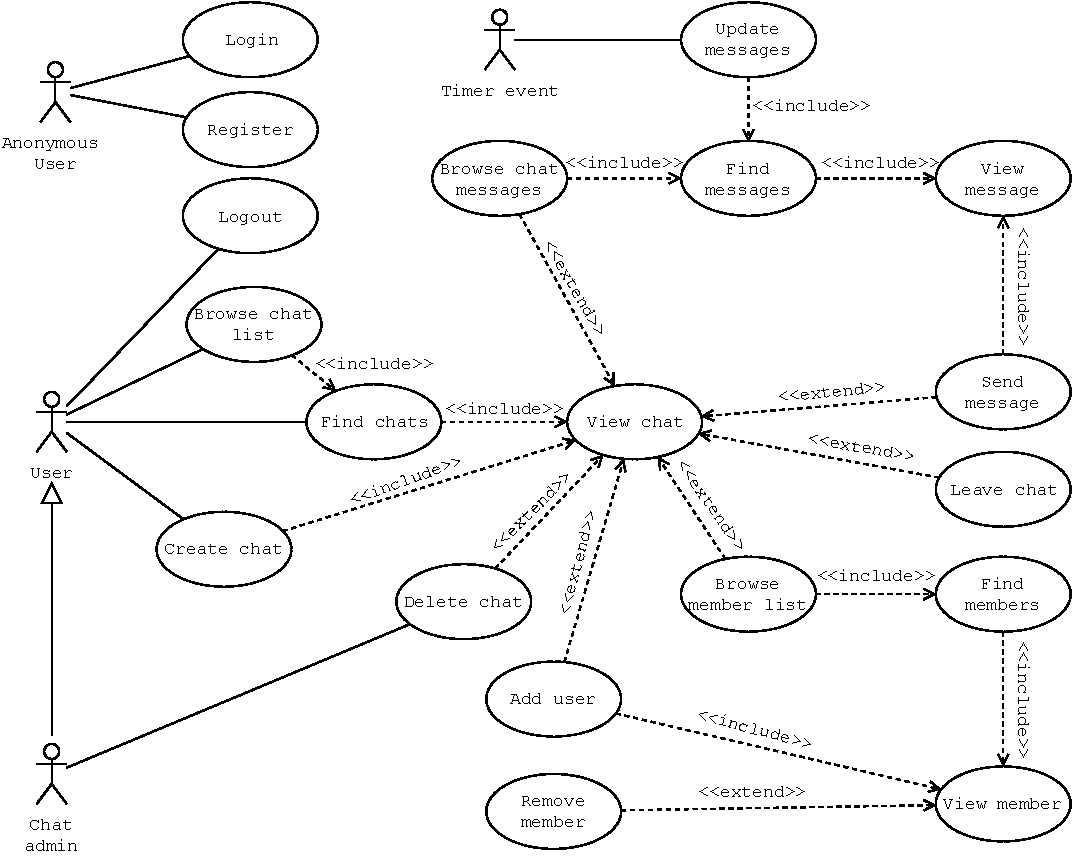
\includegraphics[width=\textwidth]{figs/use_case_diagram}
    \caption{Use-case diagram}
    \label{fig:usecase}
\end{figure}

An \textbf{anonymous user} must be able to register in order to become a 
\emph{registered user}.

A \textbf{registered user} must be able to:
\begin{itemize}
    \item Send a message to a chat
    \item Read chat messages
    \item Create a private chat
    \item Create a group chat
\end{itemize}

A \textbf{group admin} must be able to:
\begin{itemize}
    \item Add users to the group
    \item Remove users from the group
\end{itemize}

The \textbf{time-based event} updates the user interface on regular intervals
to show new received messages from the current chat, if any.

\subsection{Software Architecture}
The proposed software architecture is a classic three-layer architecture:
\begin{enumerate}
    \item database (MySQL)
    \item server back-end (Java + Spring)
    \item user web app (ReactJS)
\end{enumerate}

\section{Implementation}

\subsection{Database}
\begin{figure}[]
    \centering
    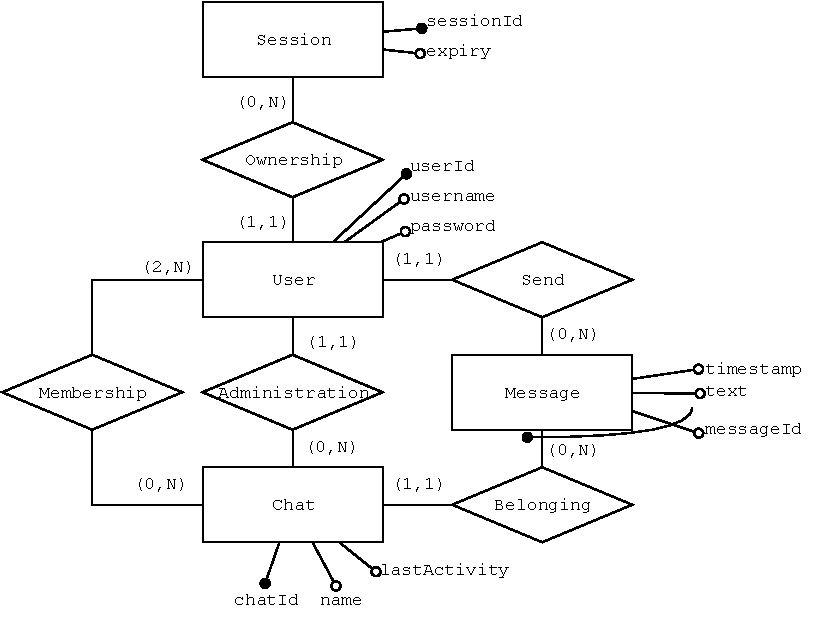
\includegraphics[width=\textwidth]{figs/ER}
    \caption{ER diagram for the database.}
    \label{fig:er}
\end{figure}

When implementing the database, we chose to keep it as simple as possible. 
That is why we did not make any distinction between \emph{private chats} and 
\emph{group chats}, creating a single \emph{Chat} entity.

Figure~\ref{fig:er} shows the ER diagram of the database. Every \emph{User} 
is identified a \emph{userId} and has got a unique \emph{username} and a 
\emph{password}. The user can be a member of many \emph{Chats} and can 
be the administrator of many \emph{Chats}. On the other hand, a \emph{Chat} 
can be administered by only one \emph{User}. A \emph{User} can send a 
\emph{Message} to a \emph{Chat}. Each \emph{User} and each \emph{Chat} can 
have many \emph{Messages} while a \emph{Message} can belong to one \emph{Chat}
and one \emph{User} only. The \emph{Session} represents a logged user session.
Each \emph{User} can have many open \emph{Sessions}.

Once the database had been created, we filled it with random test data using the free
service available at \url{http://filldb.info/}. Generated data is not perfect, 
since some more complex functional constrainst could not be included in the 
generation. However, that was sufficient for the first functional tests of the
application.

\subsection{Java backend}
Lo sviluppo e' continuando con il set-up delle dipendenze Java (Spring Boot, JDBC, Junit e Google Gson), poi sono state scritte le prime funzioni che utilizzavano il database e, allo stesso tempo, fornivano delle API accessibili tramite una richiesta HTTP di tipo appropriato. Non avendo a disposizione un frontend con cui effettuare le prove di funzionamento, e' stato utilizzato `curl` scegliendo manualmente il tipo di richiesta e i dati da inviare.
Il lavoro si e' poi diviso tra lo sviluppo della webapp React e la scrittura del Database Adapter e delle API.

Un problema che si e' posto dopo l'inizio dello sviluppo fronted riguardava il mantenimento della sessione. Si e' scelto di utilizzare un token, sessionId, generato da funzioni crittograficamente sicure e in maniera completamente pseudo-randomica (non viene utilizzato username, userId o altri dati per la generazione del token). Il sessionId, dalla validita' di 5 giorni, viene generato e inviato all'utente una volta che questo completa, con successo, il login. Le richieste effettuate dall'utente loggato conterranno tutte il sessionId come uno dei parametri. Lato server, la tabella "Sessions" mantiene l'associazione (userId, sessionId). All'arrivo di ogni richiesta effettuabile solo da utente registrato, il sessionId viene letto, viene cercato nel database e una specifica funzione ritorna lo userId che viene poi utilizzato per effettuare la relativa richiesta.


Dal lato sicurezza, al momento le password nel database sono in chiaro, sia perche' sono state generate in questo modo nei dummy data, sia per comodita' di sviluppo (utilizzando un account generato automaticamente, altrimenti, con la password hashed, non sarebbe stato possibile utilizzarlo). In produzione, si dovrebbe introdurre una funzione di hashing, come ad esempio puo' esserla SHA-256. Il tipo relativo alla password nel database e' un VARCHAR(64) esattamente per questo motivo.

\subsection{ReactJS frontend}
Per quanto riguarda il frontend, si e' fatto di uso di librerie molto comuni, evitando di entrare troppo nel dettaglio.
La struttura della pagina e' stata ottenuta tramite l'utilizzo della libreria Bootstrap.

L'evento time-based riguarda l'aggiornamento delle chat e dei messaggi.
Ogni secondo viene richiesto al server l'invio di tutte le chat di cui l'utente fa parte, ordinate per ultima attivita', in modo tale che risulti come prima chat quella con un messaggio inviato piu' di recente oppure creata da poco.
Ogni 500ms viene inviata una richiesta al server per controllare l'esistenza di nuovi messaggi. Poiche' la mole dei messaggi e', in un contesto reale, innumerevole volte piu' grande del numero delle chat, la richiesta comporta un carico non indifferente sul server. Per questo motivo, la funzione di controllo messaggi permette di specificare un timestamp da cui partire e/o un numero massimo di messaggi da ricevere.
Una piccola considerazione: il carico sul server resta comunque elevato e delle modifiche per alleggerirlo sono possibili, per questo motivo riteniamo che ci sia ancora molto margine di miglioramento sotto questo aspetto.



\end{document}
